% Options for packages loaded elsewhere
\PassOptionsToPackage{unicode}{hyperref}
\PassOptionsToPackage{hyphens}{url}
%
\documentclass[
]{article}
\usepackage{amsmath,amssymb}
\usepackage{lmodern}
\usepackage{ifxetex,ifluatex}
\ifnum 0\ifxetex 1\fi\ifluatex 1\fi=0 % if pdftex
  \usepackage[T1]{fontenc}
  \usepackage[utf8]{inputenc}
  \usepackage{textcomp} % provide euro and other symbols
\else % if luatex or xetex
  \usepackage{unicode-math}
  \defaultfontfeatures{Scale=MatchLowercase}
  \defaultfontfeatures[\rmfamily]{Ligatures=TeX,Scale=1}
\fi
% Use upquote if available, for straight quotes in verbatim environments
\IfFileExists{upquote.sty}{\usepackage{upquote}}{}
\IfFileExists{microtype.sty}{% use microtype if available
  \usepackage[]{microtype}
  \UseMicrotypeSet[protrusion]{basicmath} % disable protrusion for tt fonts
}{}
\makeatletter
\@ifundefined{KOMAClassName}{% if non-KOMA class
  \IfFileExists{parskip.sty}{%
    \usepackage{parskip}
  }{% else
    \setlength{\parindent}{0pt}
    \setlength{\parskip}{6pt plus 2pt minus 1pt}}
}{% if KOMA class
  \KOMAoptions{parskip=half}}
\makeatother
\usepackage{xcolor}
\IfFileExists{xurl.sty}{\usepackage{xurl}}{} % add URL line breaks if available
\IfFileExists{bookmark.sty}{\usepackage{bookmark}}{\usepackage{hyperref}}
\hypersetup{
  pdftitle={Homework 4},
  hidelinks,
  pdfcreator={LaTeX via pandoc}}
\urlstyle{same} % disable monospaced font for URLs
\usepackage[margin=1in]{geometry}
\usepackage{color}
\usepackage{fancyvrb}
\newcommand{\VerbBar}{|}
\newcommand{\VERB}{\Verb[commandchars=\\\{\}]}
\DefineVerbatimEnvironment{Highlighting}{Verbatim}{commandchars=\\\{\}}
% Add ',fontsize=\small' for more characters per line
\usepackage{framed}
\definecolor{shadecolor}{RGB}{248,248,248}
\newenvironment{Shaded}{\begin{snugshade}}{\end{snugshade}}
\newcommand{\AlertTok}[1]{\textcolor[rgb]{0.94,0.16,0.16}{#1}}
\newcommand{\AnnotationTok}[1]{\textcolor[rgb]{0.56,0.35,0.01}{\textbf{\textit{#1}}}}
\newcommand{\AttributeTok}[1]{\textcolor[rgb]{0.77,0.63,0.00}{#1}}
\newcommand{\BaseNTok}[1]{\textcolor[rgb]{0.00,0.00,0.81}{#1}}
\newcommand{\BuiltInTok}[1]{#1}
\newcommand{\CharTok}[1]{\textcolor[rgb]{0.31,0.60,0.02}{#1}}
\newcommand{\CommentTok}[1]{\textcolor[rgb]{0.56,0.35,0.01}{\textit{#1}}}
\newcommand{\CommentVarTok}[1]{\textcolor[rgb]{0.56,0.35,0.01}{\textbf{\textit{#1}}}}
\newcommand{\ConstantTok}[1]{\textcolor[rgb]{0.00,0.00,0.00}{#1}}
\newcommand{\ControlFlowTok}[1]{\textcolor[rgb]{0.13,0.29,0.53}{\textbf{#1}}}
\newcommand{\DataTypeTok}[1]{\textcolor[rgb]{0.13,0.29,0.53}{#1}}
\newcommand{\DecValTok}[1]{\textcolor[rgb]{0.00,0.00,0.81}{#1}}
\newcommand{\DocumentationTok}[1]{\textcolor[rgb]{0.56,0.35,0.01}{\textbf{\textit{#1}}}}
\newcommand{\ErrorTok}[1]{\textcolor[rgb]{0.64,0.00,0.00}{\textbf{#1}}}
\newcommand{\ExtensionTok}[1]{#1}
\newcommand{\FloatTok}[1]{\textcolor[rgb]{0.00,0.00,0.81}{#1}}
\newcommand{\FunctionTok}[1]{\textcolor[rgb]{0.00,0.00,0.00}{#1}}
\newcommand{\ImportTok}[1]{#1}
\newcommand{\InformationTok}[1]{\textcolor[rgb]{0.56,0.35,0.01}{\textbf{\textit{#1}}}}
\newcommand{\KeywordTok}[1]{\textcolor[rgb]{0.13,0.29,0.53}{\textbf{#1}}}
\newcommand{\NormalTok}[1]{#1}
\newcommand{\OperatorTok}[1]{\textcolor[rgb]{0.81,0.36,0.00}{\textbf{#1}}}
\newcommand{\OtherTok}[1]{\textcolor[rgb]{0.56,0.35,0.01}{#1}}
\newcommand{\PreprocessorTok}[1]{\textcolor[rgb]{0.56,0.35,0.01}{\textit{#1}}}
\newcommand{\RegionMarkerTok}[1]{#1}
\newcommand{\SpecialCharTok}[1]{\textcolor[rgb]{0.00,0.00,0.00}{#1}}
\newcommand{\SpecialStringTok}[1]{\textcolor[rgb]{0.31,0.60,0.02}{#1}}
\newcommand{\StringTok}[1]{\textcolor[rgb]{0.31,0.60,0.02}{#1}}
\newcommand{\VariableTok}[1]{\textcolor[rgb]{0.00,0.00,0.00}{#1}}
\newcommand{\VerbatimStringTok}[1]{\textcolor[rgb]{0.31,0.60,0.02}{#1}}
\newcommand{\WarningTok}[1]{\textcolor[rgb]{0.56,0.35,0.01}{\textbf{\textit{#1}}}}
\usepackage{graphicx}
\makeatletter
\def\maxwidth{\ifdim\Gin@nat@width>\linewidth\linewidth\else\Gin@nat@width\fi}
\def\maxheight{\ifdim\Gin@nat@height>\textheight\textheight\else\Gin@nat@height\fi}
\makeatother
% Scale images if necessary, so that they will not overflow the page
% margins by default, and it is still possible to overwrite the defaults
% using explicit options in \includegraphics[width, height, ...]{}
\setkeys{Gin}{width=\maxwidth,height=\maxheight,keepaspectratio}
% Set default figure placement to htbp
\makeatletter
\def\fps@figure{htbp}
\makeatother
\setlength{\emergencystretch}{3em} % prevent overfull lines
\providecommand{\tightlist}{%
  \setlength{\itemsep}{0pt}\setlength{\parskip}{0pt}}
\setcounter{secnumdepth}{-\maxdimen} % remove section numbering
\ifluatex
  \usepackage{selnolig}  % disable illegal ligatures
\fi

\title{Homework 4}
\author{}
\date{\vspace{-2.5em}}

\begin{document}
\maketitle

Part 2. This needs to be submitted by Sunday 24th on Canvas as an Rmd
and a rendered file.

\begin{Shaded}
\begin{Highlighting}[]
\FunctionTok{library}\NormalTok{(tidyverse)}
\end{Highlighting}
\end{Shaded}

\begin{verbatim}
## -- Attaching packages --------------------------------------- tidyverse 1.3.1 --
\end{verbatim}

\begin{verbatim}
## v ggplot2 3.3.5     v purrr   0.3.4
## v tibble  3.1.6     v dplyr   1.0.7
## v tidyr   1.1.4     v stringr 1.4.0
## v readr   2.0.1     v forcats 0.5.1
\end{verbatim}

\begin{verbatim}
## -- Conflicts ------------------------------------------ tidyverse_conflicts() --
## x dplyr::filter() masks stats::filter()
## x dplyr::lag()    masks stats::lag()
\end{verbatim}

\begin{Shaded}
\begin{Highlighting}[]
\FunctionTok{library}\NormalTok{(dplyr)}
\FunctionTok{library}\NormalTok{(readxl)}
\end{Highlighting}
\end{Shaded}

In this homework, you will have to work with the experiment data we
collected for this class.

\begin{enumerate}
\def\labelenumi{\arabic{enumi}.}
\item
  \textbf{\texttt{We\ are\ interested\ in\ whether\ some\ people\ were\ more\ likely\ to\ make\ correct\ guesses.\ What\ are\ the\ summary\ statistics\ for\ all\ draws?\ Plot\ a\ histogram.\ Are\ there\ any\ outliers\ in\ the\ data\ (i.e.\ individuals\ who\ guess\ 0\ times\ correctly\ and\ individuals\ who\ guessed\ all\ 20\ times\ correctly?)}}

  \textbf{we draw a histogram based on the summary statistics. To find}

\begin{Shaded}
\begin{Highlighting}[]
\FunctionTok{library}\NormalTok{(readxl)}
\NormalTok{exp21 }\OtherTok{\textless{}{-}} \FunctionTok{read\_excel}\NormalTok{(}\StringTok{"experiment\_2021C(1)copy.xlsx"}\NormalTok{, }\AttributeTok{col\_names =} \ConstantTok{FALSE}\NormalTok{,}
    \AttributeTok{skip =} \DecValTok{2}\NormalTok{)}
\end{Highlighting}
\end{Shaded}

\begin{verbatim}
## New names:
## * `` -> ...1
## * `` -> ...2
## * `` -> ...3
## * `` -> ...4
## * `` -> ...5
## * ...
\end{verbatim}

  I find all the outcome columns and I name them after the variable
  names of our dataset.

\begin{Shaded}
\begin{Highlighting}[]
\NormalTok{var\_names }\OtherTok{\textless{}{-}} \FunctionTok{read\_excel}\NormalTok{(}\StringTok{"experiment\_2021C(1)copy.xlsx"}\NormalTok{, }\AttributeTok{n\_max =} \DecValTok{1}\NormalTok{) }
\end{Highlighting}
\end{Shaded}

\begin{verbatim}
## New names:
## * `Q171_First Click` -> `Q171_First Click...46`
## * `Q171_Last Click` -> `Q171_Last Click...47`
## * `Q171_Page Submit` -> `Q171_Page Submit...48`
## * `Q171_Click Count` -> `Q171_Click Count...49`
## * `Q171_First Click` -> `Q171_First Click...82`
## * ...
\end{verbatim}

\begin{Shaded}
\begin{Highlighting}[]
\FunctionTok{colnames}\NormalTok{(exp21) }\OtherTok{\textless{}{-}} \FunctionTok{colnames}\NormalTok{(var\_names)}

\FunctionTok{rm}\NormalTok{(var\_names) }

\NormalTok{columnss }\OtherTok{\textless{}{-}}\NormalTok{ exp21 }\SpecialCharTok{\%\textgreater{}\%} 
  \FunctionTok{select}\NormalTok{(}\FunctionTok{starts\_with}\NormalTok{(}\StringTok{"Outcome"}\NormalTok{), }\StringTok{"Age"}\NormalTok{, }\StringTok{"Risk"}\NormalTok{, }\StringTok{"Gender"}\NormalTok{, }\StringTok{"SC0"}\NormalTok{) }
\end{Highlighting}
\end{Shaded}

  Now we pivot longer to have all the outcomes in line. This helps to
  name the correct answers as ``1'' and the wrong answers as ``0''.

\begin{Shaded}
\begin{Highlighting}[]
\NormalTok{countcol }\OtherTok{\textless{}{-}}\NormalTok{ columnss }\SpecialCharTok{\%\textgreater{}\%} 
  \FunctionTok{pivot\_longer}\NormalTok{(}\AttributeTok{cols =} \FunctionTok{starts\_with}\NormalTok{(}\StringTok{"Outcome"}\NormalTok{), }\AttributeTok{names\_to=} \StringTok{"draw"}\NormalTok{, }\AttributeTok{values\_to =} \StringTok{"answer"}\NormalTok{) }\SpecialCharTok{\%\textgreater{}\%}
  \FunctionTok{mutate}\NormalTok{(}\AttributeTok{count=} \FunctionTok{case\_when}\NormalTok{(answer }\SpecialCharTok{==} \StringTok{"Yes (bonus payment of $0.10)"} \SpecialCharTok{\textasciitilde{}} \DecValTok{1}\NormalTok{,}
\NormalTok{         answer }\SpecialCharTok{==} \StringTok{"No (no bonus payment)"} \SpecialCharTok{\textasciitilde{}} \DecValTok{0}\NormalTok{))}
\end{Highlighting}
\end{Shaded}

  After we pivot wider back in its first format. This helps us to have
  the data

\begin{Shaded}
\begin{Highlighting}[]
\NormalTok{pilpi }\OtherTok{\textless{}{-}}\NormalTok{ countcol }\SpecialCharTok{\%\textgreater{}\%} \FunctionTok{select}\NormalTok{(}\SpecialCharTok{{-}}\NormalTok{answer) }\SpecialCharTok{\%\textgreater{}\%} \FunctionTok{mutate}\NormalTok{(}\AttributeTok{id =} \FunctionTok{rep}\NormalTok{(}\DecValTok{1}\SpecialCharTok{:}\DecValTok{133}\NormalTok{, }\AttributeTok{each =} \DecValTok{20}\NormalTok{)) }\SpecialCharTok{\%\textgreater{}\%}  \FunctionTok{pivot\_wider}\NormalTok{(}\AttributeTok{id\_cols =} \FunctionTok{c}\NormalTok{(id, Age, SC0, Risk, Gender), }\AttributeTok{names\_from =}\NormalTok{ draw, }\AttributeTok{values\_from =}\NormalTok{ count)}
\end{Highlighting}
\end{Shaded}

  We use pivot longer once more in order to have all the observations in
  one column. Having the observations in one column, is easier for us to
  group by the id column we created before. So we groupby id. This helps
  us identify what each person done. In addition, we add a column using
  mutate in order to have the clear result of each person.

\begin{Shaded}
\begin{Highlighting}[]
\NormalTok{pi }\OtherTok{\textless{}{-}}\NormalTok{ pilpi }\SpecialCharTok{\%\textgreater{}\%} \FunctionTok{pivot\_longer}\NormalTok{(}\AttributeTok{cols =} \FunctionTok{starts\_with}\NormalTok{(}\StringTok{"Outcome"}\NormalTok{), }\AttributeTok{names\_to=} \StringTok{"draw"}\NormalTok{, }\AttributeTok{values\_to =} \StringTok{"answer"}\NormalTok{) }\SpecialCharTok{\%\textgreater{}\%} \FunctionTok{group\_by}\NormalTok{(id) }

\NormalTok{ti}\OtherTok{\textless{}{-}}\NormalTok{ pi }\SpecialCharTok{\%\textgreater{}\%} \FunctionTok{mutate}\NormalTok{(}\AttributeTok{summm=}\FunctionTok{sum}\NormalTok{(answer))}

\NormalTok{tii}\OtherTok{\textless{}{-}}\NormalTok{ pi }\SpecialCharTok{\%\textgreater{}\%} \FunctionTok{mutate}\NormalTok{(}\AttributeTok{summm=}\FunctionTok{sum}\NormalTok{(answer)) }\SpecialCharTok{\%\textgreater{}\%} \FunctionTok{separate}\NormalTok{(draw, }\AttributeTok{into =} \FunctionTok{c}\NormalTok{(}\StringTok{"rolsep"}\NormalTok{, }\StringTok{"rolnum"}\NormalTok{), }\AttributeTok{sep =} \StringTok{"e"}\NormalTok{) }\SpecialCharTok{\%\textgreater{}\%} \FunctionTok{group\_by}\NormalTok{(id)}

\CommentTok{\# boxplot.stats(data$score)$out}
\CommentTok{\# }
\CommentTok{\# rr \textless{}{-} ti \%\textgreater{}\% separate(draw, into = c("rolsep", "rolnum"), sep = "e") \%\textgreater{}\% group\_by(id, rolnum)}
\end{Highlighting}
\end{Shaded}

  Now we pivot wider once more so the data can be presented in the form
  that shows how people are doing from the 1st one until the last
  (133rd).

\begin{Shaded}
\begin{Highlighting}[]
\NormalTok{final }\OtherTok{\textless{}{-}}\NormalTok{ ti }\SpecialCharTok{\%\textgreater{}\%}  \FunctionTok{pivot\_wider}\NormalTok{(}\AttributeTok{id\_cols =} \FunctionTok{c}\NormalTok{(id, Age, SC0, Risk, Gender, summm), }\AttributeTok{names\_from =}\NormalTok{ draw, }\AttributeTok{values\_from =}\NormalTok{ answer)}

\CommentTok{\# finally \textless{}{-} tii \%\textgreater{}\%  pivot\_wider(id\_cols = c(id, Age, SC0, Risk, Gender, summm), names\_from = rolnum, values\_from = answer)}
\CommentTok{\# }
\CommentTok{\#   fin \textless{}{-} final \%\textgreater{}\% inner\_join(ex22, by = "id")}
\end{Highlighting}
\end{Shaded}

  We use the code below to do our Histogram.

\begin{Shaded}
\begin{Highlighting}[]
\FunctionTok{ggplot}\NormalTok{(final, }\FunctionTok{aes}\NormalTok{(summm)) }\SpecialCharTok{+} \FunctionTok{geom\_histogram}\NormalTok{(}\AttributeTok{bins =} \DecValTok{21}\NormalTok{) }\SpecialCharTok{+} \FunctionTok{geom\_rug}\NormalTok{()}
\end{Highlighting}
\end{Shaded}

  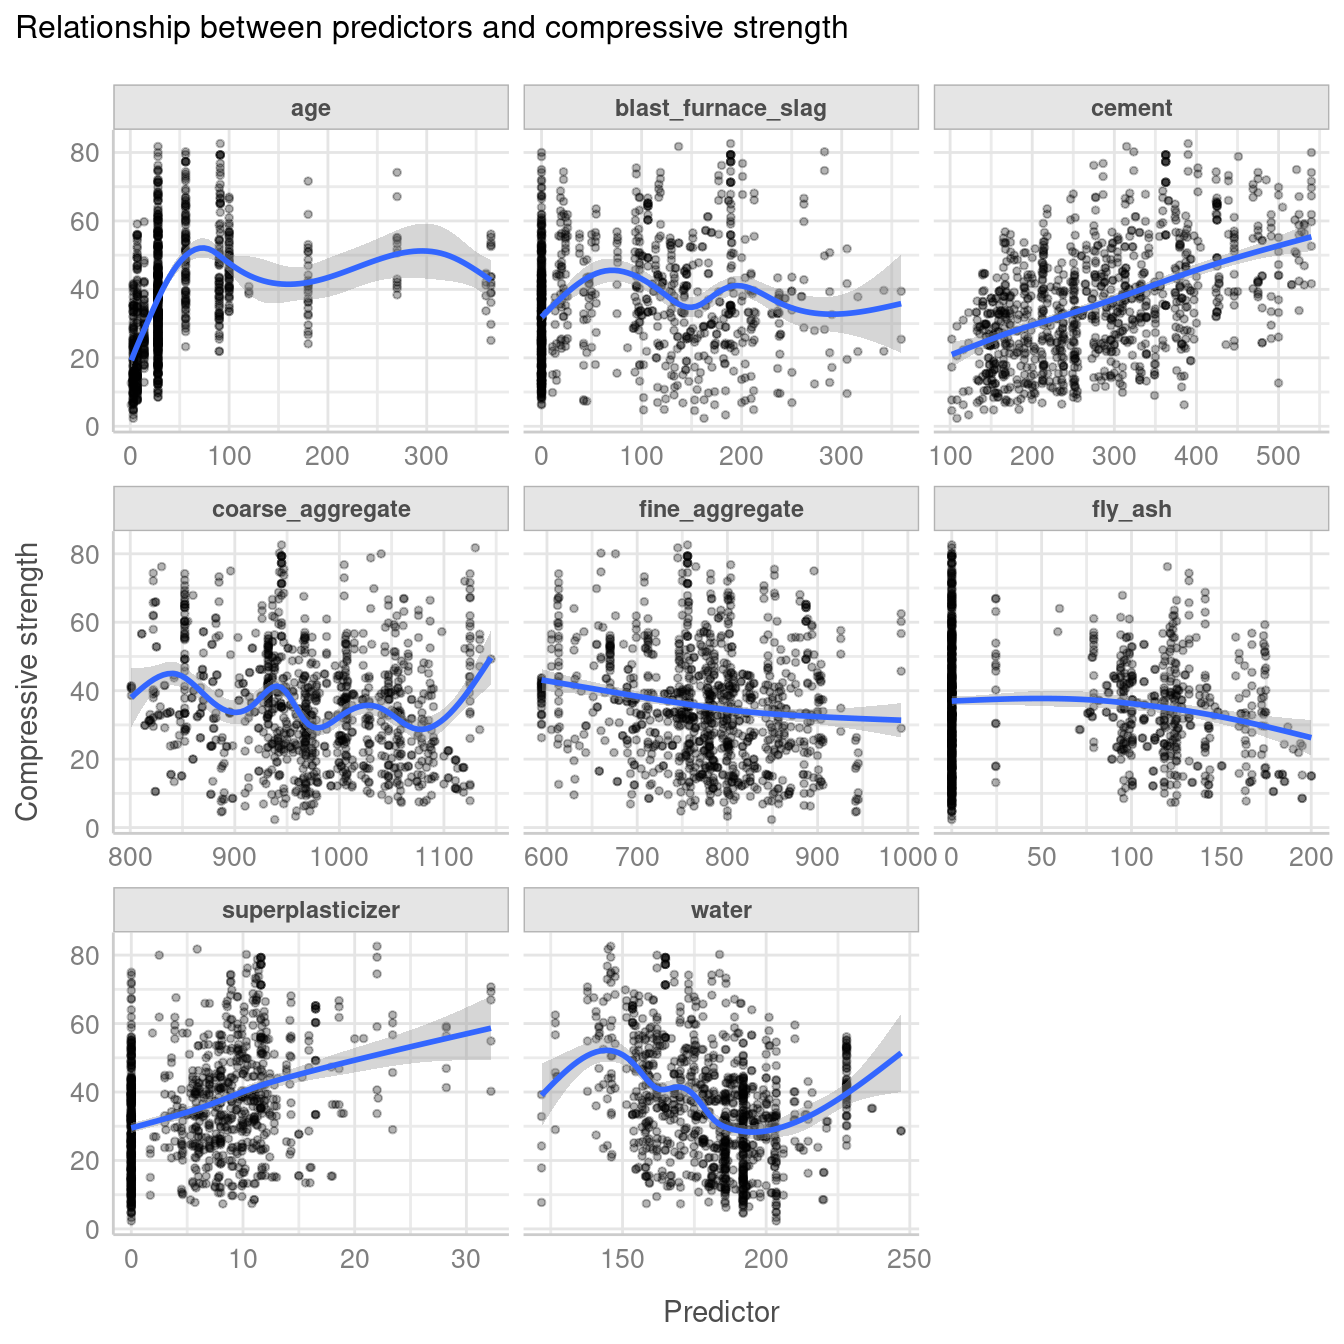
\includegraphics{H4_files/figure-latex/unnamed-chunk-8-1.pdf}
\item
  \textbf{\texttt{Analyze\ the\ data\ by\ gender,\ the\ draw\ number,\ and\ by\ experimental\ condition.\ Are\ there\ differences\ between\ the\ genders\ in\ terms\ of\ the\ number\ of\ wins\ versus\ losses?\ Are\ there\ differences\ between\ the\ experimental\ conditions?\ Are\ people\ more\ or\ less\ likely\ to\ win\ towards\ the\ last\ draws\ as\ opposed\ to\ the\ beginning\ of\ the\ experiment?}}

  `Final' is the column that already has everything needed for the
  analysis. The only missing column is conditions. To do that, I used
  mutate to create a new column named as condition where each real
  condition is named after a number from one to five. I also create an
  id column in the ex2 dataset so I can then inner\_join it with our
  main column.

\begin{Shaded}
\begin{Highlighting}[]
\NormalTok{ex2 }\OtherTok{\textless{}{-}}\NormalTok{ exp21 }\SpecialCharTok{\%\textgreater{}\%}
         \FunctionTok{mutate}\NormalTok{(}\AttributeTok{condition =} \FunctionTok{case\_when}\NormalTok{(Control\_Msg }\SpecialCharTok{!=} \StringTok{""} \SpecialCharTok{\textasciitilde{}} \DecValTok{1}\NormalTok{,}
\NormalTok{                               Norm\_Pos\_Msg }\SpecialCharTok{!=} \StringTok{""} \SpecialCharTok{\textasciitilde{}} \DecValTok{2}\NormalTok{,}
\NormalTok{                               Norm\_Neg\_Msg }\SpecialCharTok{!=} \StringTok{""} \SpecialCharTok{\textasciitilde{}} \DecValTok{3}\NormalTok{,}
\NormalTok{                               Emp\_Neg\_Msg }\SpecialCharTok{!=} \StringTok{""} \SpecialCharTok{\textasciitilde{}} \DecValTok{4}\NormalTok{,}
\NormalTok{                               Emp\_Pos\_Msg }\SpecialCharTok{!=} \StringTok{""} \SpecialCharTok{\textasciitilde{}} \DecValTok{5}\NormalTok{),}
                \AttributeTok{id =} \DecValTok{1}\SpecialCharTok{:}\DecValTok{133}\NormalTok{,}
                \AttributeTok{rolnum =} \DecValTok{1}\SpecialCharTok{:}\DecValTok{133}\NormalTok{) }
\end{Highlighting}
\end{Shaded}

  At this point, I create a new dataset with `id' and `condition'
  columns so it is easier to inner\_join them. Then I inner\_join them
  so I have everything in one dataset named `fin'.

\begin{Shaded}
\begin{Highlighting}[]
\NormalTok{ex22 }\OtherTok{\textless{}{-}}\NormalTok{ ex2 }\SpecialCharTok{\%\textgreater{}\%} \FunctionTok{select}\NormalTok{(id, condition, rolnum)}

\NormalTok{fin }\OtherTok{\textless{}{-}}\NormalTok{ final }\SpecialCharTok{\%\textgreater{}\%} \FunctionTok{inner\_join}\NormalTok{(ex22, }\AttributeTok{by =} \StringTok{"id"}\NormalTok{)}
\end{Highlighting}
\end{Shaded}

  Then we group by Gender and summarise by mean. This allows us to see
  the mean score that each gender got correct. As we can see, females
  reported a higher correct score than males on average.

\begin{Shaded}
\begin{Highlighting}[]
\NormalTok{fin }\SpecialCharTok{\%\textgreater{}\%} \FunctionTok{group\_by}\NormalTok{(Gender) }\SpecialCharTok{\%\textgreater{}\%} \FunctionTok{summarise}\NormalTok{(}\FunctionTok{mean}\NormalTok{(summm))}
\end{Highlighting}
\end{Shaded}

\begin{verbatim}
## # A tibble: 2 x 2
##   Gender `mean(summm)`
##   <chr>          <dbl>
## 1 Female          4.75
## 2 Male            3.68
\end{verbatim}

\begin{Shaded}
\begin{Highlighting}[]
\CommentTok{\# mutate(rrr, coun)}
\CommentTok{\# fin \%\textgreater{}\% group\_by(condition) \%\textgreater{}\% summarise(mean(summm))}
\end{Highlighting}
\end{Shaded}

  Analyzing the data regarding the draw number we use the tii dataset.
  The reason is because this dataset was created in question 1 with a
  function named seperate. This function separated the column `draw'
  into two others (rolsep, rolsum). The first stands for the title of
  the draw column while the second one stands for the values that a
  correct answer was reported.

  Therefore, we here use the filter column(rolnum) equal with the number
  of observation we want piped with summary(answer). This helps us find
  the stats behind the correct answers in each round. Also, we named a
  new dataset `i' where it excludes some irrelevant columns for the
  purpose of analyzing the data based on draws.

  Regarding the draws we can see that the mean for outcome number 1 is
  almost 20\% (0.1955). That means that one out of five people reported
  a correct answer in that case. As we can see the mean of correct
  responses ranges from 0.16 to 0.27. This means that the standard
  deviation is relatively low. In other words all correct response rates
  are clustered around the mean.

\begin{Shaded}
\begin{Highlighting}[]
\NormalTok{i }\OtherTok{\textless{}{-}}\NormalTok{ tii }\SpecialCharTok{\%\textgreater{}\%} \FunctionTok{select}\NormalTok{(}\SpecialCharTok{{-}}\NormalTok{Gender, }\SpecialCharTok{{-}}\NormalTok{Age, }\SpecialCharTok{{-}}\NormalTok{SC0, }\SpecialCharTok{{-}}\NormalTok{id, }\SpecialCharTok{{-}}\NormalTok{Risk, }\SpecialCharTok{{-}}\NormalTok{rolsep, }\SpecialCharTok{{-}}\NormalTok{summm, }\SpecialCharTok{{-}}\NormalTok{id)}
\end{Highlighting}
\end{Shaded}

\begin{verbatim}
## Adding missing grouping variables: `id`
\end{verbatim}

\begin{Shaded}
\begin{Highlighting}[]
\NormalTok{i }\SpecialCharTok{\%\textgreater{}\%} \FunctionTok{filter}\NormalTok{(rolnum}\SpecialCharTok{==}\DecValTok{1}\NormalTok{) }\SpecialCharTok{\%\textgreater{}\%} \FunctionTok{summary}\NormalTok{(answer)}
\end{Highlighting}
\end{Shaded}

\begin{verbatim}
##        id         rolnum              answer      
##  Min.   :  1   Length:133         Min.   :0.0000  
##  1st Qu.: 34   Class :character   1st Qu.:0.0000  
##  Median : 67   Mode  :character   Median :0.0000  
##  Mean   : 67                      Mean   :0.1955  
##  3rd Qu.:100                      3rd Qu.:0.0000  
##  Max.   :133                      Max.   :1.0000
\end{verbatim}

\begin{Shaded}
\begin{Highlighting}[]
\NormalTok{i }\SpecialCharTok{\%\textgreater{}\%} \FunctionTok{filter}\NormalTok{(rolnum}\SpecialCharTok{==}\DecValTok{2}\NormalTok{) }\SpecialCharTok{\%\textgreater{}\%} \FunctionTok{summary}\NormalTok{(answer)}
\end{Highlighting}
\end{Shaded}

\begin{verbatim}
##        id         rolnum              answer      
##  Min.   :  1   Length:133         Min.   :0.0000  
##  1st Qu.: 34   Class :character   1st Qu.:0.0000  
##  Median : 67   Mode  :character   Median :0.0000  
##  Mean   : 67                      Mean   :0.2406  
##  3rd Qu.:100                      3rd Qu.:0.0000  
##  Max.   :133                      Max.   :1.0000
\end{verbatim}

\begin{Shaded}
\begin{Highlighting}[]
\NormalTok{i }\SpecialCharTok{\%\textgreater{}\%} \FunctionTok{filter}\NormalTok{(rolnum}\SpecialCharTok{==}\DecValTok{3}\NormalTok{) }\SpecialCharTok{\%\textgreater{}\%} \FunctionTok{summary}\NormalTok{(answer)}
\end{Highlighting}
\end{Shaded}

\begin{verbatim}
##        id         rolnum              answer      
##  Min.   :  1   Length:133         Min.   :0.0000  
##  1st Qu.: 34   Class :character   1st Qu.:0.0000  
##  Median : 67   Mode  :character   Median :0.0000  
##  Mean   : 67                      Mean   :0.1654  
##  3rd Qu.:100                      3rd Qu.:0.0000  
##  Max.   :133                      Max.   :1.0000
\end{verbatim}

\begin{Shaded}
\begin{Highlighting}[]
\NormalTok{i }\SpecialCharTok{\%\textgreater{}\%} \FunctionTok{filter}\NormalTok{(rolnum}\SpecialCharTok{==}\DecValTok{4}\NormalTok{) }\SpecialCharTok{\%\textgreater{}\%} \FunctionTok{summary}\NormalTok{(answer)}
\end{Highlighting}
\end{Shaded}

\begin{verbatim}
##        id         rolnum              answer      
##  Min.   :  1   Length:133         Min.   :0.0000  
##  1st Qu.: 34   Class :character   1st Qu.:0.0000  
##  Median : 67   Mode  :character   Median :0.0000  
##  Mean   : 67                      Mean   :0.1654  
##  3rd Qu.:100                      3rd Qu.:0.0000  
##  Max.   :133                      Max.   :1.0000
\end{verbatim}

\begin{Shaded}
\begin{Highlighting}[]
\NormalTok{i }\SpecialCharTok{\%\textgreater{}\%} \FunctionTok{filter}\NormalTok{(rolnum}\SpecialCharTok{==}\DecValTok{5}\NormalTok{) }\SpecialCharTok{\%\textgreater{}\%} \FunctionTok{summary}\NormalTok{(answer)}
\end{Highlighting}
\end{Shaded}

\begin{verbatim}
##        id         rolnum              answer      
##  Min.   :  1   Length:133         Min.   :0.0000  
##  1st Qu.: 34   Class :character   1st Qu.:0.0000  
##  Median : 67   Mode  :character   Median :0.0000  
##  Mean   : 67                      Mean   :0.2331  
##  3rd Qu.:100                      3rd Qu.:0.0000  
##  Max.   :133                      Max.   :1.0000
\end{verbatim}

\begin{Shaded}
\begin{Highlighting}[]
\NormalTok{i }\SpecialCharTok{\%\textgreater{}\%} \FunctionTok{filter}\NormalTok{(rolnum}\SpecialCharTok{==}\DecValTok{6}\NormalTok{) }\SpecialCharTok{\%\textgreater{}\%} \FunctionTok{summary}\NormalTok{(answer)}
\end{Highlighting}
\end{Shaded}

\begin{verbatim}
##        id         rolnum              answer      
##  Min.   :  1   Length:133         Min.   :0.0000  
##  1st Qu.: 34   Class :character   1st Qu.:0.0000  
##  Median : 67   Mode  :character   Median :0.0000  
##  Mean   : 67                      Mean   :0.2556  
##  3rd Qu.:100                      3rd Qu.:1.0000  
##  Max.   :133                      Max.   :1.0000
\end{verbatim}

\begin{Shaded}
\begin{Highlighting}[]
\NormalTok{i }\SpecialCharTok{\%\textgreater{}\%} \FunctionTok{filter}\NormalTok{(rolnum}\SpecialCharTok{==}\DecValTok{7}\NormalTok{) }\SpecialCharTok{\%\textgreater{}\%} \FunctionTok{summary}\NormalTok{(answer)}
\end{Highlighting}
\end{Shaded}

\begin{verbatim}
##        id         rolnum              answer     
##  Min.   :  1   Length:133         Min.   :0.000  
##  1st Qu.: 34   Class :character   1st Qu.:0.000  
##  Median : 67   Mode  :character   Median :0.000  
##  Mean   : 67                      Mean   :0.203  
##  3rd Qu.:100                      3rd Qu.:0.000  
##  Max.   :133                      Max.   :1.000
\end{verbatim}

\begin{Shaded}
\begin{Highlighting}[]
\NormalTok{i }\SpecialCharTok{\%\textgreater{}\%} \FunctionTok{filter}\NormalTok{(rolnum}\SpecialCharTok{==}\DecValTok{8}\NormalTok{) }\SpecialCharTok{\%\textgreater{}\%} \FunctionTok{summary}\NormalTok{(answer)}
\end{Highlighting}
\end{Shaded}

\begin{verbatim}
##        id         rolnum              answer      
##  Min.   :  1   Length:133         Min.   :0.0000  
##  1st Qu.: 34   Class :character   1st Qu.:0.0000  
##  Median : 67   Mode  :character   Median :0.0000  
##  Mean   : 67                      Mean   :0.1955  
##  3rd Qu.:100                      3rd Qu.:0.0000  
##  Max.   :133                      Max.   :1.0000
\end{verbatim}

\begin{Shaded}
\begin{Highlighting}[]
\NormalTok{i }\SpecialCharTok{\%\textgreater{}\%} \FunctionTok{filter}\NormalTok{(rolnum}\SpecialCharTok{==}\DecValTok{9}\NormalTok{) }\SpecialCharTok{\%\textgreater{}\%} \FunctionTok{summary}\NormalTok{(answer)}
\end{Highlighting}
\end{Shaded}

\begin{verbatim}
##        id         rolnum              answer      
##  Min.   :  1   Length:133         Min.   :0.0000  
##  1st Qu.: 34   Class :character   1st Qu.:0.0000  
##  Median : 67   Mode  :character   Median :0.0000  
##  Mean   : 67                      Mean   :0.2406  
##  3rd Qu.:100                      3rd Qu.:0.0000  
##  Max.   :133                      Max.   :1.0000
\end{verbatim}

\begin{Shaded}
\begin{Highlighting}[]
\NormalTok{i }\SpecialCharTok{\%\textgreater{}\%} \FunctionTok{filter}\NormalTok{(rolnum}\SpecialCharTok{==}\DecValTok{10}\NormalTok{) }\SpecialCharTok{\%\textgreater{}\%} \FunctionTok{summary}\NormalTok{(answer)}
\end{Highlighting}
\end{Shaded}

\begin{verbatim}
##        id         rolnum              answer      
##  Min.   :  1   Length:133         Min.   :0.0000  
##  1st Qu.: 34   Class :character   1st Qu.:0.0000  
##  Median : 67   Mode  :character   Median :0.0000  
##  Mean   : 67                      Mean   :0.2105  
##  3rd Qu.:100                      3rd Qu.:0.0000  
##  Max.   :133                      Max.   :1.0000
\end{verbatim}

\begin{Shaded}
\begin{Highlighting}[]
\NormalTok{i }\SpecialCharTok{\%\textgreater{}\%} \FunctionTok{filter}\NormalTok{(rolnum}\SpecialCharTok{==}\DecValTok{11}\NormalTok{) }\SpecialCharTok{\%\textgreater{}\%} \FunctionTok{summary}\NormalTok{(answer)}
\end{Highlighting}
\end{Shaded}

\begin{verbatim}
##        id         rolnum              answer     
##  Min.   :  1   Length:133         Min.   :0.000  
##  1st Qu.: 34   Class :character   1st Qu.:0.000  
##  Median : 67   Mode  :character   Median :0.000  
##  Mean   : 67                      Mean   :0.203  
##  3rd Qu.:100                      3rd Qu.:0.000  
##  Max.   :133                      Max.   :1.000
\end{verbatim}

\begin{Shaded}
\begin{Highlighting}[]
\NormalTok{i }\SpecialCharTok{\%\textgreater{}\%} \FunctionTok{filter}\NormalTok{(rolnum}\SpecialCharTok{==}\DecValTok{12}\NormalTok{) }\SpecialCharTok{\%\textgreater{}\%} \FunctionTok{summary}\NormalTok{(answer)}
\end{Highlighting}
\end{Shaded}

\begin{verbatim}
##        id         rolnum              answer      
##  Min.   :  1   Length:133         Min.   :0.0000  
##  1st Qu.: 34   Class :character   1st Qu.:0.0000  
##  Median : 67   Mode  :character   Median :0.0000  
##  Mean   : 67                      Mean   :0.1955  
##  3rd Qu.:100                      3rd Qu.:0.0000  
##  Max.   :133                      Max.   :1.0000
\end{verbatim}

\begin{Shaded}
\begin{Highlighting}[]
\NormalTok{i }\SpecialCharTok{\%\textgreater{}\%} \FunctionTok{filter}\NormalTok{(rolnum}\SpecialCharTok{==}\DecValTok{13}\NormalTok{) }\SpecialCharTok{\%\textgreater{}\%} \FunctionTok{summary}\NormalTok{(answer)}
\end{Highlighting}
\end{Shaded}

\begin{verbatim}
##        id         rolnum              answer      
##  Min.   :  1   Length:133         Min.   :0.0000  
##  1st Qu.: 34   Class :character   1st Qu.:0.0000  
##  Median : 67   Mode  :character   Median :0.0000  
##  Mean   : 67                      Mean   :0.1955  
##  3rd Qu.:100                      3rd Qu.:0.0000  
##  Max.   :133                      Max.   :1.0000
\end{verbatim}

\begin{Shaded}
\begin{Highlighting}[]
\NormalTok{i }\SpecialCharTok{\%\textgreater{}\%} \FunctionTok{filter}\NormalTok{(rolnum}\SpecialCharTok{==}\DecValTok{14}\NormalTok{) }\SpecialCharTok{\%\textgreater{}\%} \FunctionTok{summary}\NormalTok{(answer)}
\end{Highlighting}
\end{Shaded}

\begin{verbatim}
##        id         rolnum              answer      
##  Min.   :  1   Length:133         Min.   :0.0000  
##  1st Qu.: 34   Class :character   1st Qu.:0.0000  
##  Median : 67   Mode  :character   Median :0.0000  
##  Mean   : 67                      Mean   :0.2707  
##  3rd Qu.:100                      3rd Qu.:1.0000  
##  Max.   :133                      Max.   :1.0000
\end{verbatim}

\begin{Shaded}
\begin{Highlighting}[]
\NormalTok{i }\SpecialCharTok{\%\textgreater{}\%} \FunctionTok{filter}\NormalTok{(rolnum}\SpecialCharTok{==}\DecValTok{15}\NormalTok{) }\SpecialCharTok{\%\textgreater{}\%} \FunctionTok{summary}\NormalTok{(answer)}
\end{Highlighting}
\end{Shaded}

\begin{verbatim}
##        id         rolnum              answer      
##  Min.   :  1   Length:133         Min.   :0.0000  
##  1st Qu.: 34   Class :character   1st Qu.:0.0000  
##  Median : 67   Mode  :character   Median :0.0000  
##  Mean   : 67                      Mean   :0.2556  
##  3rd Qu.:100                      3rd Qu.:1.0000  
##  Max.   :133                      Max.   :1.0000
\end{verbatim}

\begin{Shaded}
\begin{Highlighting}[]
\NormalTok{i }\SpecialCharTok{\%\textgreater{}\%} \FunctionTok{filter}\NormalTok{(rolnum}\SpecialCharTok{==}\DecValTok{16}\NormalTok{) }\SpecialCharTok{\%\textgreater{}\%} \FunctionTok{summary}\NormalTok{(answer)}
\end{Highlighting}
\end{Shaded}

\begin{verbatim}
##        id         rolnum              answer      
##  Min.   :  1   Length:133         Min.   :0.0000  
##  1st Qu.: 34   Class :character   1st Qu.:0.0000  
##  Median : 67   Mode  :character   Median :0.0000  
##  Mean   : 67                      Mean   :0.2556  
##  3rd Qu.:100                      3rd Qu.:1.0000  
##  Max.   :133                      Max.   :1.0000
\end{verbatim}

\begin{Shaded}
\begin{Highlighting}[]
\NormalTok{i }\SpecialCharTok{\%\textgreater{}\%} \FunctionTok{filter}\NormalTok{(rolnum}\SpecialCharTok{==}\DecValTok{17}\NormalTok{) }\SpecialCharTok{\%\textgreater{}\%} \FunctionTok{summary}\NormalTok{(answer)}
\end{Highlighting}
\end{Shaded}

\begin{verbatim}
##        id         rolnum              answer      
##  Min.   :  1   Length:133         Min.   :0.0000  
##  1st Qu.: 34   Class :character   1st Qu.:0.0000  
##  Median : 67   Mode  :character   Median :0.0000  
##  Mean   : 67                      Mean   :0.2256  
##  3rd Qu.:100                      3rd Qu.:0.0000  
##  Max.   :133                      Max.   :1.0000
\end{verbatim}

\begin{Shaded}
\begin{Highlighting}[]
\NormalTok{i }\SpecialCharTok{\%\textgreater{}\%} \FunctionTok{filter}\NormalTok{(rolnum}\SpecialCharTok{==}\DecValTok{18}\NormalTok{) }\SpecialCharTok{\%\textgreater{}\%} \FunctionTok{summary}\NormalTok{(answer)}
\end{Highlighting}
\end{Shaded}

\begin{verbatim}
##        id         rolnum              answer      
##  Min.   :  1   Length:133         Min.   :0.0000  
##  1st Qu.: 34   Class :character   1st Qu.:0.0000  
##  Median : 67   Mode  :character   Median :0.0000  
##  Mean   : 67                      Mean   :0.2105  
##  3rd Qu.:100                      3rd Qu.:0.0000  
##  Max.   :133                      Max.   :1.0000
\end{verbatim}

\begin{Shaded}
\begin{Highlighting}[]
\NormalTok{i }\SpecialCharTok{\%\textgreater{}\%} \FunctionTok{filter}\NormalTok{(rolnum}\SpecialCharTok{==}\DecValTok{19}\NormalTok{) }\SpecialCharTok{\%\textgreater{}\%} \FunctionTok{summary}\NormalTok{(answer)}
\end{Highlighting}
\end{Shaded}

\begin{verbatim}
##        id         rolnum              answer     
##  Min.   :  1   Length:133         Min.   :0.000  
##  1st Qu.: 34   Class :character   1st Qu.:0.000  
##  Median : 67   Mode  :character   Median :0.000  
##  Mean   : 67                      Mean   :0.218  
##  3rd Qu.:100                      3rd Qu.:0.000  
##  Max.   :133                      Max.   :1.000
\end{verbatim}

\begin{Shaded}
\begin{Highlighting}[]
\NormalTok{i }\SpecialCharTok{\%\textgreater{}\%} \FunctionTok{filter}\NormalTok{(rolnum}\SpecialCharTok{==}\DecValTok{20}\NormalTok{) }\SpecialCharTok{\%\textgreater{}\%} \FunctionTok{summary}\NormalTok{(answer)}
\end{Highlighting}
\end{Shaded}

\begin{verbatim}
##        id         rolnum              answer      
##  Min.   :  1   Length:133         Min.   :0.0000  
##  1st Qu.: 34   Class :character   1st Qu.:0.0000  
##  Median : 67   Mode  :character   Median :0.0000  
##  Mean   : 67                      Mean   :0.2632  
##  3rd Qu.:100                      3rd Qu.:1.0000  
##  Max.   :133                      Max.   :1.0000
\end{verbatim}

  Regarding the experimental condition of the data, we use the groupby
  function to call it in the fin dataset, and then use summarise to find
  the mean. Alongside, as we set above, each number corresponds in one
  condition. As we can see, the most popular experimental condition is
  normative positive message (2) while the least popular is empirical
  positive message (5).

\begin{Shaded}
\begin{Highlighting}[]
\NormalTok{fin }\SpecialCharTok{\%\textgreater{}\%} \FunctionTok{group\_by}\NormalTok{(condition) }\SpecialCharTok{\%\textgreater{}\%} \FunctionTok{summarise}\NormalTok{(}\FunctionTok{mean}\NormalTok{(summm))}
\end{Highlighting}
\end{Shaded}

\begin{verbatim}
## # A tibble: 5 x 2
##   condition `mean(summm)`
##       <dbl>         <dbl>
## 1         1          5.52
## 2         2          6.08
## 3         3          4.20
## 4         4          3.64
## 5         5          3.36
\end{verbatim}
\item
  \textbf{\texttt{Redo\ part\ 2\ after\ excluding\ outliers.\ Do\ you\ still\ see\ the\ different\ in\ the\ experimental\ groups\ after\ outliers\ are\ eliminated?\ Do\ you\ see\ differences\ between\ the\ first\ and\ the\ last\ rolls?\ Are\ there\ any\ differences\ by\ gender?}}

\begin{Shaded}
\begin{Highlighting}[]
\CommentTok{\# trial \textless{}{-} fin \%\textgreater{}\% select({-}Gender, {-}Age, {-}SC0, {-}Risk, {-}Outcome1, {-}Outcome2, {-}Outcome3, {-}Outcome4, {-}Outcome5, {-}Outcome6, {-}Outcome7, {-}Outcome8, {-}Outcome9, {-}Outcome10, {-}Outcome11, {-}Outcome12, {-}Outcome13, {-}Outcome14, {-}Outcome15, {-}Outcome16, {-}Outcome17, {-}Outcome18, {-}Outcome19, {-}Outcome20, {-}rolnum) \%\textgreater{}\% }
\CommentTok{\#   boxplot(trial)}
\CommentTok{\# }
\CommentTok{\# boxplot.stats(trial$summm)$out }
\end{Highlighting}
\end{Shaded}

\begin{Shaded}
\begin{Highlighting}[]
\FunctionTok{boxplot}\NormalTok{(fin}\SpecialCharTok{$}\NormalTok{summm,}
  \AttributeTok{ylab =} \StringTok{"summm"}\NormalTok{)}
\end{Highlighting}
\end{Shaded}

  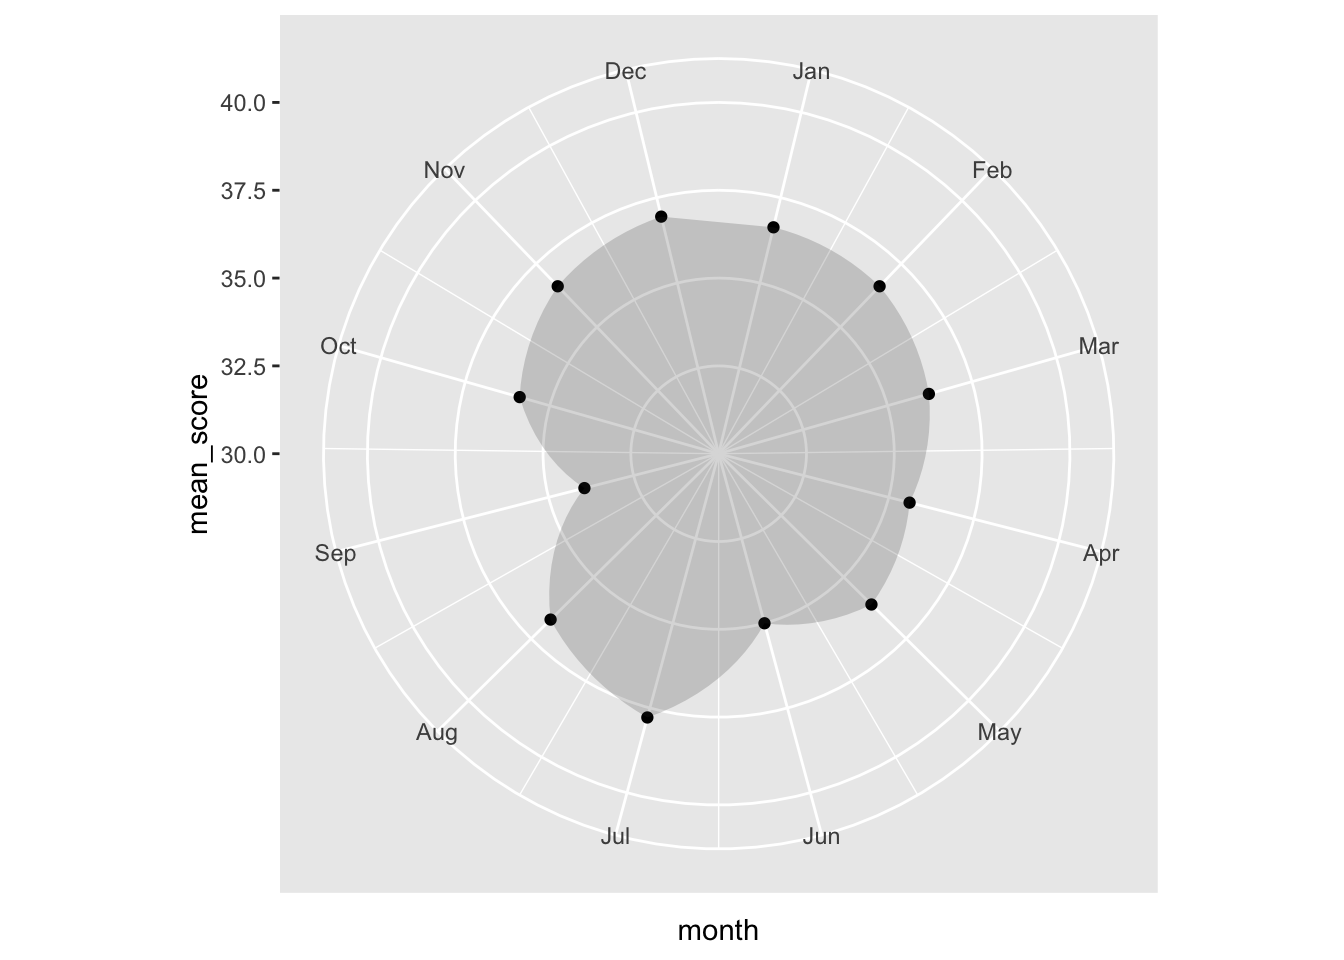
\includegraphics{H4_files/figure-latex/unnamed-chunk-15-1.pdf}

\begin{Shaded}
\begin{Highlighting}[]
\FunctionTok{boxplot.stats}\NormalTok{(fin}\SpecialCharTok{$}\NormalTok{summm)}\SpecialCharTok{$}\NormalTok{out}
\end{Highlighting}
\end{Shaded}

\begin{verbatim}
## [1] 10 17 20 11 13 10 11 13
\end{verbatim}

\begin{Shaded}
\begin{Highlighting}[]
\NormalTok{out }\OtherTok{\textless{}{-}} \FunctionTok{boxplot.stats}\NormalTok{(fin}\SpecialCharTok{$}\NormalTok{summm)}\SpecialCharTok{$}\NormalTok{out}
\NormalTok{out\_ind }\OtherTok{\textless{}{-}} \FunctionTok{which}\NormalTok{(fin}\SpecialCharTok{$}\NormalTok{summm }\SpecialCharTok{\%in\%} \FunctionTok{c}\NormalTok{(out))}
\NormalTok{out\_ind}
\end{Highlighting}
\end{Shaded}

\begin{verbatim}
## [1]  15  25  48  57  89  98 121 130
\end{verbatim}

\begin{Shaded}
\begin{Highlighting}[]
\CommentTok{\# ggplot(fin) +}
\CommentTok{\#   aes(x = summm) +}
\CommentTok{\#   geom\_histogram(bins = 21, fill = "\#0c4c8a") +}
\CommentTok{\#   theme\_minimal()}
\end{Highlighting}
\end{Shaded}

  After, wecreate a new dataset called `desperate' where we remove the
  indicative rows with the outliers. This will help us redo exercise 2

\begin{Shaded}
\begin{Highlighting}[]
\NormalTok{desperate }\OtherTok{\textless{}{-}}\NormalTok{ fin[}\SpecialCharTok{{-}}\FunctionTok{c}\NormalTok{(}\DecValTok{15}\NormalTok{, }\DecValTok{25}\NormalTok{,}\DecValTok{48}\NormalTok{,}\DecValTok{57}\NormalTok{,}\DecValTok{89}\NormalTok{,}\DecValTok{98}\NormalTok{,}\DecValTok{121}\NormalTok{,}\DecValTok{130}\NormalTok{), ]}
\end{Highlighting}
\end{Shaded}

  \textbf{Redoing exercise 2 with the new dataframe `desperate'.}

  In comparison with exercise 2, we can see that the mean for both male
  and female has fallen. This was a natural outcome to follow since the
  outliers were all above the mean. However, the outcome remained the
  same in matters of which gender reported the most correct answers. On
  average females report 4 correct answers out of twenty, as opposed to
  men (3/20).

\begin{Shaded}
\begin{Highlighting}[]
\NormalTok{desperate }\SpecialCharTok{\%\textgreater{}\%} \FunctionTok{group\_by}\NormalTok{(Gender) }\SpecialCharTok{\%\textgreater{}\%} \FunctionTok{summarise}\NormalTok{(}\FunctionTok{mean}\NormalTok{(summm))}
\end{Highlighting}
\end{Shaded}

\begin{verbatim}
## # A tibble: 2 x 2
##   Gender `mean(summm)`
##   <chr>          <dbl>
## 1 Female          4.19
## 2 Male            3.14
\end{verbatim}

  For the draws, we are creating a new column to make the analysis named
  `abcdefg'. This is to exclude the outlier rows from the the `tii'
  dataset we've used at exercise 2. After doing that though, we can see
  that the mean correct response reporting ratio remained at the same
  levels ranging from 16.54\% to 27.07\%. This indicates that the
  outliers did not affect the variability of the data. No difference
  between the first and last rows.

\begin{Shaded}
\begin{Highlighting}[]
\NormalTok{abcdefg }\OtherTok{\textless{}{-}}\NormalTok{ tii[}\SpecialCharTok{{-}}\FunctionTok{c}\NormalTok{(}\DecValTok{15}\NormalTok{, }\DecValTok{25}\NormalTok{,}\DecValTok{48}\NormalTok{,}\DecValTok{57}\NormalTok{,}\DecValTok{89}\NormalTok{,}\DecValTok{98}\NormalTok{,}\DecValTok{121}\NormalTok{,}\DecValTok{130}\NormalTok{), ]}

\NormalTok{i }\OtherTok{\textless{}{-}}\NormalTok{ abcdefg }\SpecialCharTok{\%\textgreater{}\%} \FunctionTok{select}\NormalTok{(}\SpecialCharTok{{-}}\NormalTok{Gender, }\SpecialCharTok{{-}}\NormalTok{Age, }\SpecialCharTok{{-}}\NormalTok{SC0, }\SpecialCharTok{{-}}\NormalTok{id, }\SpecialCharTok{{-}}\NormalTok{Risk, }\SpecialCharTok{{-}}\NormalTok{summm, }\SpecialCharTok{{-}}\NormalTok{rolsep, }\SpecialCharTok{{-}}\NormalTok{id)}
\end{Highlighting}
\end{Shaded}

\begin{verbatim}
## Adding missing grouping variables: `id`
\end{verbatim}

\begin{Shaded}
\begin{Highlighting}[]
\NormalTok{i }\SpecialCharTok{\%\textgreater{}\%} \FunctionTok{filter}\NormalTok{(rolnum}\SpecialCharTok{==}\DecValTok{1}\NormalTok{) }\SpecialCharTok{\%\textgreater{}\%} \FunctionTok{summary}\NormalTok{(answer)}
\end{Highlighting}
\end{Shaded}

\begin{verbatim}
##        id            rolnum              answer     
##  Min.   :  1.00   Length:132         Min.   :0.000  
##  1st Qu.: 34.75   Class :character   1st Qu.:0.000  
##  Median : 67.50   Mode  :character   Median :0.000  
##  Mean   : 67.45                      Mean   :0.197  
##  3rd Qu.:100.25                      3rd Qu.:0.000  
##  Max.   :133.00                      Max.   :1.000
\end{verbatim}

\begin{Shaded}
\begin{Highlighting}[]
\NormalTok{i }\SpecialCharTok{\%\textgreater{}\%} \FunctionTok{filter}\NormalTok{(rolnum}\SpecialCharTok{==}\DecValTok{2}\NormalTok{) }\SpecialCharTok{\%\textgreater{}\%} \FunctionTok{summary}\NormalTok{(answer)}
\end{Highlighting}
\end{Shaded}

\begin{verbatim}
##        id         rolnum              answer      
##  Min.   :  1   Length:133         Min.   :0.0000  
##  1st Qu.: 34   Class :character   1st Qu.:0.0000  
##  Median : 67   Mode  :character   Median :0.0000  
##  Mean   : 67                      Mean   :0.2406  
##  3rd Qu.:100                      3rd Qu.:0.0000  
##  Max.   :133                      Max.   :1.0000
\end{verbatim}

\begin{Shaded}
\begin{Highlighting}[]
\NormalTok{i }\SpecialCharTok{\%\textgreater{}\%} \FunctionTok{filter}\NormalTok{(rolnum}\SpecialCharTok{==}\DecValTok{3}\NormalTok{) }\SpecialCharTok{\%\textgreater{}\%} \FunctionTok{summary}\NormalTok{(answer)}
\end{Highlighting}
\end{Shaded}

\begin{verbatim}
##        id         rolnum              answer      
##  Min.   :  1   Length:133         Min.   :0.0000  
##  1st Qu.: 34   Class :character   1st Qu.:0.0000  
##  Median : 67   Mode  :character   Median :0.0000  
##  Mean   : 67                      Mean   :0.1654  
##  3rd Qu.:100                      3rd Qu.:0.0000  
##  Max.   :133                      Max.   :1.0000
\end{verbatim}

\begin{Shaded}
\begin{Highlighting}[]
\NormalTok{i }\SpecialCharTok{\%\textgreater{}\%} \FunctionTok{filter}\NormalTok{(rolnum}\SpecialCharTok{==}\DecValTok{4}\NormalTok{) }\SpecialCharTok{\%\textgreater{}\%} \FunctionTok{summary}\NormalTok{(answer)}
\end{Highlighting}
\end{Shaded}

\begin{verbatim}
##        id         rolnum              answer      
##  Min.   :  1   Length:133         Min.   :0.0000  
##  1st Qu.: 34   Class :character   1st Qu.:0.0000  
##  Median : 67   Mode  :character   Median :0.0000  
##  Mean   : 67                      Mean   :0.1654  
##  3rd Qu.:100                      3rd Qu.:0.0000  
##  Max.   :133                      Max.   :1.0000
\end{verbatim}

\begin{Shaded}
\begin{Highlighting}[]
\NormalTok{i }\SpecialCharTok{\%\textgreater{}\%} \FunctionTok{filter}\NormalTok{(rolnum}\SpecialCharTok{==}\DecValTok{5}\NormalTok{) }\SpecialCharTok{\%\textgreater{}\%} \FunctionTok{summary}\NormalTok{(answer)}
\end{Highlighting}
\end{Shaded}

\begin{verbatim}
##        id            rolnum              answer      
##  Min.   :  1.00   Length:132         Min.   :0.0000  
##  1st Qu.: 34.75   Class :character   1st Qu.:0.0000  
##  Median : 67.50   Mode  :character   Median :0.0000  
##  Mean   : 67.49                      Mean   :0.2348  
##  3rd Qu.:100.25                      3rd Qu.:0.0000  
##  Max.   :133.00                      Max.   :1.0000
\end{verbatim}

\begin{Shaded}
\begin{Highlighting}[]
\NormalTok{i }\SpecialCharTok{\%\textgreater{}\%} \FunctionTok{filter}\NormalTok{(rolnum}\SpecialCharTok{==}\DecValTok{6}\NormalTok{) }\SpecialCharTok{\%\textgreater{}\%} \FunctionTok{summary}\NormalTok{(answer)}
\end{Highlighting}
\end{Shaded}

\begin{verbatim}
##        id         rolnum              answer      
##  Min.   :  1   Length:133         Min.   :0.0000  
##  1st Qu.: 34   Class :character   1st Qu.:0.0000  
##  Median : 67   Mode  :character   Median :0.0000  
##  Mean   : 67                      Mean   :0.2556  
##  3rd Qu.:100                      3rd Qu.:1.0000  
##  Max.   :133                      Max.   :1.0000
\end{verbatim}

\begin{Shaded}
\begin{Highlighting}[]
\NormalTok{i }\SpecialCharTok{\%\textgreater{}\%} \FunctionTok{filter}\NormalTok{(rolnum}\SpecialCharTok{==}\DecValTok{7}\NormalTok{) }\SpecialCharTok{\%\textgreater{}\%} \FunctionTok{summary}\NormalTok{(answer)}
\end{Highlighting}
\end{Shaded}

\begin{verbatim}
##        id         rolnum              answer     
##  Min.   :  1   Length:133         Min.   :0.000  
##  1st Qu.: 34   Class :character   1st Qu.:0.000  
##  Median : 67   Mode  :character   Median :0.000  
##  Mean   : 67                      Mean   :0.203  
##  3rd Qu.:100                      3rd Qu.:0.000  
##  Max.   :133                      Max.   :1.000
\end{verbatim}

\begin{Shaded}
\begin{Highlighting}[]
\NormalTok{i }\SpecialCharTok{\%\textgreater{}\%} \FunctionTok{filter}\NormalTok{(rolnum}\SpecialCharTok{==}\DecValTok{8}\NormalTok{) }\SpecialCharTok{\%\textgreater{}\%} \FunctionTok{summary}\NormalTok{(answer)}
\end{Highlighting}
\end{Shaded}

\begin{verbatim}
##        id            rolnum              answer     
##  Min.   :  1.00   Length:132         Min.   :0.000  
##  1st Qu.: 34.75   Class :character   1st Qu.:0.000  
##  Median : 67.50   Mode  :character   Median :0.000  
##  Mean   : 67.48                      Mean   :0.197  
##  3rd Qu.:100.25                      3rd Qu.:0.000  
##  Max.   :133.00                      Max.   :1.000
\end{verbatim}

\begin{Shaded}
\begin{Highlighting}[]
\NormalTok{i }\SpecialCharTok{\%\textgreater{}\%} \FunctionTok{filter}\NormalTok{(rolnum}\SpecialCharTok{==}\DecValTok{9}\NormalTok{) }\SpecialCharTok{\%\textgreater{}\%} \FunctionTok{summary}\NormalTok{(answer)}
\end{Highlighting}
\end{Shaded}

\begin{verbatim}
##        id            rolnum              answer      
##  Min.   :  1.00   Length:132         Min.   :0.0000  
##  1st Qu.: 34.75   Class :character   1st Qu.:0.0000  
##  Median : 67.50   Mode  :character   Median :0.0000  
##  Mean   : 67.47                      Mean   :0.2348  
##  3rd Qu.:100.25                      3rd Qu.:0.0000  
##  Max.   :133.00                      Max.   :1.0000
\end{verbatim}

\begin{Shaded}
\begin{Highlighting}[]
\NormalTok{i }\SpecialCharTok{\%\textgreater{}\%} \FunctionTok{filter}\NormalTok{(rolnum}\SpecialCharTok{==}\DecValTok{10}\NormalTok{) }\SpecialCharTok{\%\textgreater{}\%} \FunctionTok{summary}\NormalTok{(answer)}
\end{Highlighting}
\end{Shaded}

\begin{verbatim}
##        id            rolnum              answer      
##  Min.   :  1.00   Length:132         Min.   :0.0000  
##  1st Qu.: 34.75   Class :character   1st Qu.:0.0000  
##  Median : 67.50   Mode  :character   Median :0.0000  
##  Mean   : 67.45                      Mean   :0.2121  
##  3rd Qu.:100.25                      3rd Qu.:0.0000  
##  Max.   :133.00                      Max.   :1.0000
\end{verbatim}

\begin{Shaded}
\begin{Highlighting}[]
\NormalTok{i }\SpecialCharTok{\%\textgreater{}\%} \FunctionTok{filter}\NormalTok{(rolnum}\SpecialCharTok{==}\DecValTok{11}\NormalTok{) }\SpecialCharTok{\%\textgreater{}\%} \FunctionTok{summary}\NormalTok{(answer)}
\end{Highlighting}
\end{Shaded}

\begin{verbatim}
##        id         rolnum              answer     
##  Min.   :  1   Length:133         Min.   :0.000  
##  1st Qu.: 34   Class :character   1st Qu.:0.000  
##  Median : 67   Mode  :character   Median :0.000  
##  Mean   : 67                      Mean   :0.203  
##  3rd Qu.:100                      3rd Qu.:0.000  
##  Max.   :133                      Max.   :1.000
\end{verbatim}

\begin{Shaded}
\begin{Highlighting}[]
\NormalTok{i }\SpecialCharTok{\%\textgreater{}\%} \FunctionTok{filter}\NormalTok{(rolnum}\SpecialCharTok{==}\DecValTok{12}\NormalTok{) }\SpecialCharTok{\%\textgreater{}\%} \FunctionTok{summary}\NormalTok{(answer)}
\end{Highlighting}
\end{Shaded}

\begin{verbatim}
##        id         rolnum              answer      
##  Min.   :  1   Length:133         Min.   :0.0000  
##  1st Qu.: 34   Class :character   1st Qu.:0.0000  
##  Median : 67   Mode  :character   Median :0.0000  
##  Mean   : 67                      Mean   :0.1955  
##  3rd Qu.:100                      3rd Qu.:0.0000  
##  Max.   :133                      Max.   :1.0000
\end{verbatim}

\begin{Shaded}
\begin{Highlighting}[]
\NormalTok{i }\SpecialCharTok{\%\textgreater{}\%} \FunctionTok{filter}\NormalTok{(rolnum}\SpecialCharTok{==}\DecValTok{13}\NormalTok{) }\SpecialCharTok{\%\textgreater{}\%} \FunctionTok{summary}\NormalTok{(answer)}
\end{Highlighting}
\end{Shaded}

\begin{verbatim}
##        id         rolnum              answer      
##  Min.   :  1   Length:133         Min.   :0.0000  
##  1st Qu.: 34   Class :character   1st Qu.:0.0000  
##  Median : 67   Mode  :character   Median :0.0000  
##  Mean   : 67                      Mean   :0.1955  
##  3rd Qu.:100                      3rd Qu.:0.0000  
##  Max.   :133                      Max.   :1.0000
\end{verbatim}

\begin{Shaded}
\begin{Highlighting}[]
\NormalTok{i }\SpecialCharTok{\%\textgreater{}\%} \FunctionTok{filter}\NormalTok{(rolnum}\SpecialCharTok{==}\DecValTok{14}\NormalTok{) }\SpecialCharTok{\%\textgreater{}\%} \FunctionTok{summary}\NormalTok{(answer)}
\end{Highlighting}
\end{Shaded}

\begin{verbatim}
##        id         rolnum              answer      
##  Min.   :  1   Length:133         Min.   :0.0000  
##  1st Qu.: 34   Class :character   1st Qu.:0.0000  
##  Median : 67   Mode  :character   Median :0.0000  
##  Mean   : 67                      Mean   :0.2707  
##  3rd Qu.:100                      3rd Qu.:1.0000  
##  Max.   :133                      Max.   :1.0000
\end{verbatim}

\begin{Shaded}
\begin{Highlighting}[]
\NormalTok{i }\SpecialCharTok{\%\textgreater{}\%} \FunctionTok{filter}\NormalTok{(rolnum}\SpecialCharTok{==}\DecValTok{15}\NormalTok{) }\SpecialCharTok{\%\textgreater{}\%} \FunctionTok{summary}\NormalTok{(answer)}
\end{Highlighting}
\end{Shaded}

\begin{verbatim}
##        id            rolnum              answer      
##  Min.   :  2.00   Length:132         Min.   :0.0000  
##  1st Qu.: 34.75   Class :character   1st Qu.:0.0000  
##  Median : 67.50   Mode  :character   Median :0.0000  
##  Mean   : 67.50                      Mean   :0.2576  
##  3rd Qu.:100.25                      3rd Qu.:1.0000  
##  Max.   :133.00                      Max.   :1.0000
\end{verbatim}

\begin{Shaded}
\begin{Highlighting}[]
\NormalTok{i }\SpecialCharTok{\%\textgreater{}\%} \FunctionTok{filter}\NormalTok{(rolnum}\SpecialCharTok{==}\DecValTok{16}\NormalTok{) }\SpecialCharTok{\%\textgreater{}\%} \FunctionTok{summary}\NormalTok{(answer)}
\end{Highlighting}
\end{Shaded}

\begin{verbatim}
##        id         rolnum              answer      
##  Min.   :  1   Length:133         Min.   :0.0000  
##  1st Qu.: 34   Class :character   1st Qu.:0.0000  
##  Median : 67   Mode  :character   Median :0.0000  
##  Mean   : 67                      Mean   :0.2556  
##  3rd Qu.:100                      3rd Qu.:1.0000  
##  Max.   :133                      Max.   :1.0000
\end{verbatim}

\begin{Shaded}
\begin{Highlighting}[]
\NormalTok{i }\SpecialCharTok{\%\textgreater{}\%} \FunctionTok{filter}\NormalTok{(rolnum}\SpecialCharTok{==}\DecValTok{17}\NormalTok{) }\SpecialCharTok{\%\textgreater{}\%} \FunctionTok{summary}\NormalTok{(answer)}
\end{Highlighting}
\end{Shaded}

\begin{verbatim}
##        id            rolnum              answer      
##  Min.   :  1.00   Length:132         Min.   :0.0000  
##  1st Qu.: 34.75   Class :character   1st Qu.:0.0000  
##  Median : 67.50   Mode  :character   Median :0.0000  
##  Mean   : 67.48                      Mean   :0.2273  
##  3rd Qu.:100.25                      3rd Qu.:0.0000  
##  Max.   :133.00                      Max.   :1.0000
\end{verbatim}

\begin{Shaded}
\begin{Highlighting}[]
\NormalTok{i }\SpecialCharTok{\%\textgreater{}\%} \FunctionTok{filter}\NormalTok{(rolnum}\SpecialCharTok{==}\DecValTok{18}\NormalTok{) }\SpecialCharTok{\%\textgreater{}\%} \FunctionTok{summary}\NormalTok{(answer)}
\end{Highlighting}
\end{Shaded}

\begin{verbatim}
##        id            rolnum              answer      
##  Min.   :  1.00   Length:132         Min.   :0.0000  
##  1st Qu.: 34.75   Class :character   1st Qu.:0.0000  
##  Median : 67.50   Mode  :character   Median :0.0000  
##  Mean   : 67.47                      Mean   :0.2045  
##  3rd Qu.:100.25                      3rd Qu.:0.0000  
##  Max.   :133.00                      Max.   :1.0000
\end{verbatim}

\begin{Shaded}
\begin{Highlighting}[]
\NormalTok{i }\SpecialCharTok{\%\textgreater{}\%} \FunctionTok{filter}\NormalTok{(rolnum}\SpecialCharTok{==}\DecValTok{19}\NormalTok{) }\SpecialCharTok{\%\textgreater{}\%} \FunctionTok{summary}\NormalTok{(answer)}
\end{Highlighting}
\end{Shaded}

\begin{verbatim}
##        id         rolnum              answer     
##  Min.   :  1   Length:133         Min.   :0.000  
##  1st Qu.: 34   Class :character   1st Qu.:0.000  
##  Median : 67   Mode  :character   Median :0.000  
##  Mean   : 67                      Mean   :0.218  
##  3rd Qu.:100                      3rd Qu.:0.000  
##  Max.   :133                      Max.   :1.000
\end{verbatim}

\begin{Shaded}
\begin{Highlighting}[]
\NormalTok{i }\SpecialCharTok{\%\textgreater{}\%} \FunctionTok{filter}\NormalTok{(rolnum}\SpecialCharTok{==}\DecValTok{20}\NormalTok{) }\SpecialCharTok{\%\textgreater{}\%} \FunctionTok{summary}\NormalTok{(answer)}
\end{Highlighting}
\end{Shaded}

\begin{verbatim}
##        id         rolnum              answer      
##  Min.   :  1   Length:133         Min.   :0.0000  
##  1st Qu.: 34   Class :character   1st Qu.:0.0000  
##  Median : 67   Mode  :character   Median :0.0000  
##  Mean   : 67                      Mean   :0.2632  
##  3rd Qu.:100                      3rd Qu.:1.0000  
##  Max.   :133                      Max.   :1.0000
\end{verbatim}

  In the case of experimental conditions we can see that there are some
  significant differences. The range between them became smaller (3.36
  to 4.69). In other words the data became more disperse. While there is
  no difference in the lower end, there is a difference in the higher
  end of the range. This indicates that the previous means were inflated
  due to the high outliers. For insance, the most popular experimental
  condition, normative positive message (2), was 6.08, whereas now is
  just 4.33.

\begin{Shaded}
\begin{Highlighting}[]
\NormalTok{desperate }\SpecialCharTok{\%\textgreater{}\%} \FunctionTok{group\_by}\NormalTok{(condition) }\SpecialCharTok{\%\textgreater{}\%} \FunctionTok{summarise}\NormalTok{(}\FunctionTok{mean}\NormalTok{(summm))}
\end{Highlighting}
\end{Shaded}

\begin{verbatim}
## # A tibble: 5 x 2
##   condition `mean(summm)`
##       <dbl>         <dbl>
## 1         1          4.70
## 2         2          4.33
## 3         3          3.74
## 4         4          3.43
## 5         5          3.36
\end{verbatim}
\item
  \texttt{Split\ your\ sample\ into\ the\ "younger"\ half\ and\ the\ "older\ half.\ Are\ there\ differences\ between\ the\ two\ age\ groups?}

  First we sort the date from highest to lowest reported age using the
  order function.
\end{enumerate}

\begin{Shaded}
\begin{Highlighting}[]
\NormalTok{ordered}\OtherTok{\textless{}{-}}\NormalTok{ fin[}\FunctionTok{order}\NormalTok{(fin}\SpecialCharTok{$}\NormalTok{Age, }\AttributeTok{decreasing =} \ConstantTok{TRUE}\NormalTok{), ]}
\end{Highlighting}
\end{Shaded}

Then we find the Age median from fin dataset. As we can see, the median
is 24 (in the column 67 since is exactly the middle of 133).

\begin{Shaded}
\begin{Highlighting}[]
\FunctionTok{median}\NormalTok{(fin}\SpecialCharTok{$}\NormalTok{Age)}
\end{Highlighting}
\end{Shaded}

\begin{verbatim}
## [1] 24
\end{verbatim}

Since I have the ordered dataframe (from the highest to lowest Age), I
use it to create two other dataframes, one for the younger Age group
``orderedyoung'', and one for the older Age group ``orderedold''.

\begin{Shaded}
\begin{Highlighting}[]
\NormalTok{orderedyoung }\OtherTok{\textless{}{-}}\NormalTok{ ordered[}\SpecialCharTok{{-}}\FunctionTok{c}\NormalTok{(}\DecValTok{1}\SpecialCharTok{:}\DecValTok{66}\NormalTok{), ]}
\NormalTok{orderedold }\OtherTok{\textless{}{-}}\NormalTok{ ordered[}\SpecialCharTok{{-}}\FunctionTok{c}\NormalTok{(}\DecValTok{68}\SpecialCharTok{:}\DecValTok{133}\NormalTok{), ]}
\end{Highlighting}
\end{Shaded}

orderedold\%\textgreater\% ggplot(aes(x= Age, y= summm)) + geom\_point()

\begin{Shaded}
\begin{Highlighting}[]
\FunctionTok{boxplot}\NormalTok{(orderedold}\SpecialCharTok{$}\NormalTok{Age,}
  \AttributeTok{ylab =} \StringTok{"Age"}\NormalTok{)}
\end{Highlighting}
\end{Shaded}

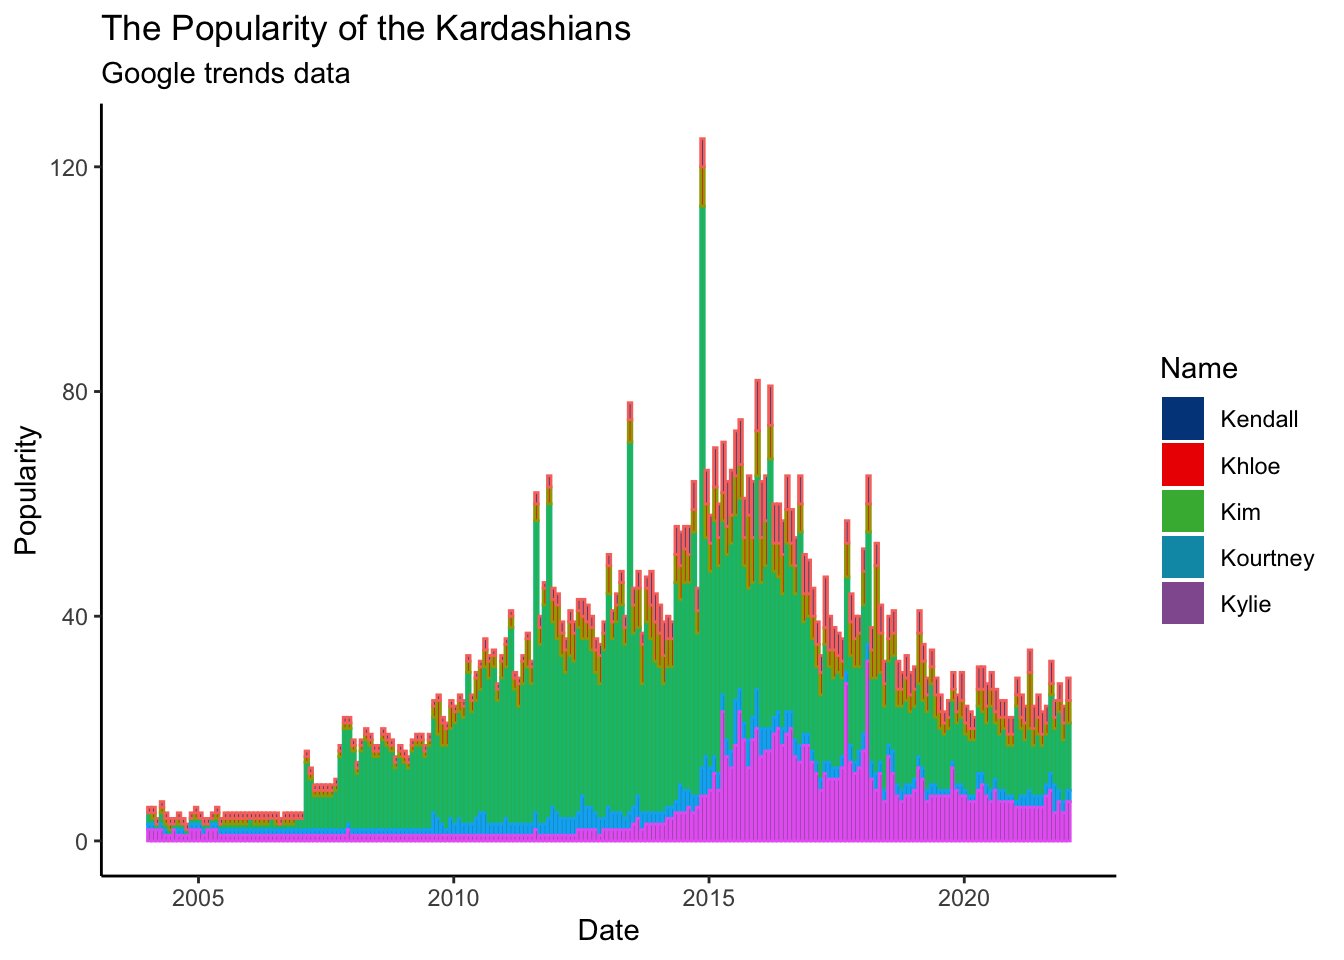
\includegraphics{H4_files/figure-latex/unnamed-chunk-23-1.pdf}

\begin{Shaded}
\begin{Highlighting}[]
\FunctionTok{boxplot.stats}\NormalTok{(orderedold}\SpecialCharTok{$}\NormalTok{Age)}\SpecialCharTok{$}\NormalTok{out}
\end{Highlighting}
\end{Shaded}

\begin{verbatim}
## [1] 56 51 46 35
\end{verbatim}

\begin{Shaded}
\begin{Highlighting}[]
\NormalTok{out }\OtherTok{\textless{}{-}} \FunctionTok{boxplot.stats}\NormalTok{(orderedold}\SpecialCharTok{$}\NormalTok{Age)}\SpecialCharTok{$}\NormalTok{out}
\NormalTok{out\_ind }\OtherTok{\textless{}{-}} \FunctionTok{which}\NormalTok{(orderedold}\SpecialCharTok{$}\NormalTok{Age }\SpecialCharTok{\%in\%} \FunctionTok{c}\NormalTok{(out))}
\NormalTok{out\_ind}
\end{Highlighting}
\end{Shaded}

\begin{verbatim}
## [1] 1 2 3 4
\end{verbatim}

\begin{Shaded}
\begin{Highlighting}[]
\FunctionTok{boxplot}\NormalTok{(orderedyoung}\SpecialCharTok{$}\NormalTok{Age,}
  \AttributeTok{ylab =} \StringTok{"Age"}\NormalTok{)}
\end{Highlighting}
\end{Shaded}

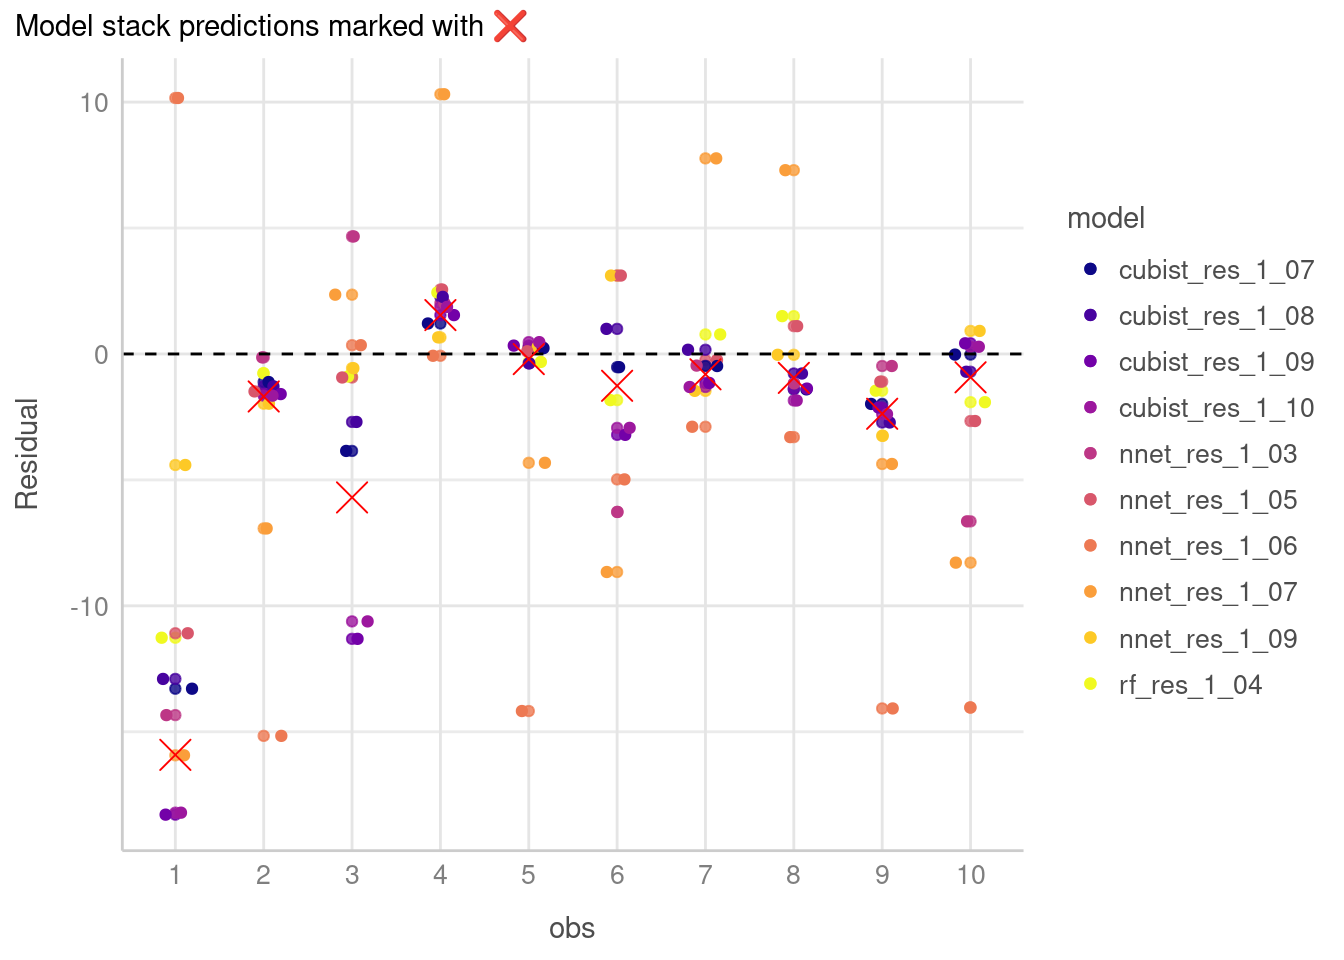
\includegraphics{H4_files/figure-latex/unnamed-chunk-24-1.pdf}

\begin{Shaded}
\begin{Highlighting}[]
\FunctionTok{boxplot.stats}\NormalTok{(orderedyoung}\SpecialCharTok{$}\NormalTok{Age)}\SpecialCharTok{$}\NormalTok{out}
\end{Highlighting}
\end{Shaded}

\begin{verbatim}
## [1] 20
\end{verbatim}

\begin{Shaded}
\begin{Highlighting}[]
\NormalTok{out }\OtherTok{\textless{}{-}} \FunctionTok{boxplot.stats}\NormalTok{(orderedyoung}\SpecialCharTok{$}\NormalTok{Age)}\SpecialCharTok{$}\NormalTok{out}
\NormalTok{out\_ind }\OtherTok{\textless{}{-}} \FunctionTok{which}\NormalTok{(orderedyoung}\SpecialCharTok{$}\NormalTok{Age }\SpecialCharTok{\%in\%} \FunctionTok{c}\NormalTok{(out))}
\NormalTok{out\_ind}
\end{Highlighting}
\end{Shaded}

\begin{verbatim}
## [1] 67
\end{verbatim}

\begin{Shaded}
\begin{Highlighting}[]
\NormalTok{oo }\OtherTok{\textless{}{-}}\NormalTok{ orderedold[}\SpecialCharTok{{-}}\FunctionTok{c}\NormalTok{(}\DecValTok{1}\NormalTok{,}\DecValTok{2}\NormalTok{,}\DecValTok{3}\NormalTok{,}\DecValTok{4}\NormalTok{), ]}

\NormalTok{oy }\OtherTok{\textless{}{-}}\NormalTok{ orderedyoung[}\SpecialCharTok{{-}}\FunctionTok{c}\NormalTok{(}\DecValTok{67}\NormalTok{), ]}
\end{Highlighting}
\end{Shaded}

I use the ggplot function to create a graph that indicates the Age of
the participants in the x axes, and the number of correct guesses
(summm) in the y axes. As we can see, while the Age column now indicates
only the oldest people, the majority is still under 30 -- closer to the
median. From the age 24 until 30s, the amount of correct responses seems
to decline. We use the median and the mean code in order to see if there
is a difference with them. Median indicates that there is no difference
among the data as the reported correct outcome. However, if we look at
the mean of the two, the younger group tends to report more correct
answers on average than the older group. This difference is small though
(4.62-3.92)

\begin{Shaded}
\begin{Highlighting}[]
\NormalTok{oo}\SpecialCharTok{\%\textgreater{}\%} \FunctionTok{ggplot}\NormalTok{(}\FunctionTok{aes}\NormalTok{(}\AttributeTok{x=}\NormalTok{ Age, }\AttributeTok{y=}\NormalTok{ summm)) }\SpecialCharTok{+} \FunctionTok{geom\_point}\NormalTok{()}
\end{Highlighting}
\end{Shaded}

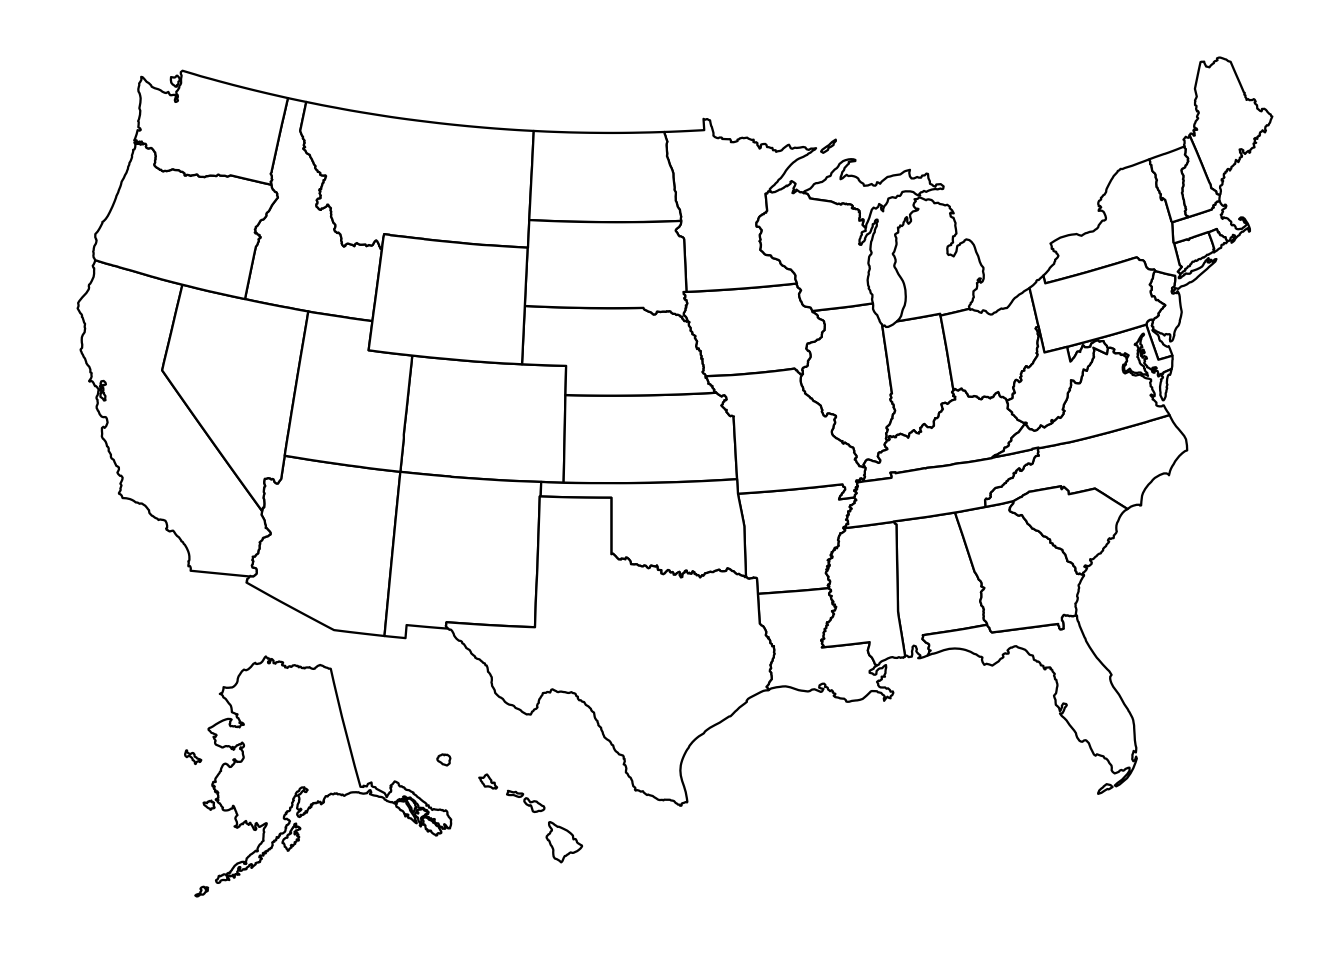
\includegraphics{H4_files/figure-latex/unnamed-chunk-26-1.pdf}

\begin{Shaded}
\begin{Highlighting}[]
\FunctionTok{median}\NormalTok{(oo}\SpecialCharTok{$}\NormalTok{summm)}
\end{Highlighting}
\end{Shaded}

\begin{verbatim}
## [1] 4
\end{verbatim}

\begin{Shaded}
\begin{Highlighting}[]
\FunctionTok{mean}\NormalTok{(oo}\SpecialCharTok{$}\NormalTok{summm)}
\end{Highlighting}
\end{Shaded}

\begin{verbatim}
## [1] 3.920635
\end{verbatim}

\begin{Shaded}
\begin{Highlighting}[]
\NormalTok{oy}\SpecialCharTok{\%\textgreater{}\%} \FunctionTok{ggplot}\NormalTok{(}\FunctionTok{aes}\NormalTok{(}\AttributeTok{x=}\NormalTok{ Age, }\AttributeTok{y=}\NormalTok{ summm)) }\SpecialCharTok{+} \FunctionTok{geom\_point}\NormalTok{()}
\end{Highlighting}
\end{Shaded}

\includegraphics{H4_files/figure-latex/unnamed-chunk-26-2.pdf}

\begin{Shaded}
\begin{Highlighting}[]
\FunctionTok{median}\NormalTok{(oy}\SpecialCharTok{$}\NormalTok{summm)}
\end{Highlighting}
\end{Shaded}

\begin{verbatim}
## [1] 4
\end{verbatim}

\begin{Shaded}
\begin{Highlighting}[]
\FunctionTok{mean}\NormalTok{(oy}\SpecialCharTok{$}\NormalTok{summm)}
\end{Highlighting}
\end{Shaded}

\begin{verbatim}
## [1] 4.621212
\end{verbatim}

\end{document}
